\documentclass{article}

\usepackage{fancyhdr}
\pagestyle{fancy}
\fancypagestyle{normal}{%
  \fancyhead{} % clear all header fields
  \fancyhead[L]{\leftmark}}
\fancypagestyle{special}{%
  \fancyhead{} % clear all header fields
  \fancyhead[L]{\rightmark}}

\renewcommand{\sectionmark}[1]{%
  \markright{\thesection.\ #1}{}}

\setlength{\headheight}{13.6pt}

\usepackage{graphicx}
\usepackage{hyperref}

\usepackage[backend=biber]{biblatex}
\addbibresource{cite.bib}

\author{Tovi}
\title{ArcheryOS}

\begin{document}

\maketitle

\tableofcontents

\pagebreak

\section{Introduction}
ArcheryOS is an arch based, rolling release, lightweight pentesting distribution. It uses the default arch linux repositories, to ensure your software is always kept up to date.
\subsection{Philosophy of ArcheryOS}
\begin{itemize}
	\item Minimal

		ArcheryOS is designed to be minimal. It comes preinstalled with i3, which is a minimal window manager (wm) that focuses on utilising as much space as possible.\ i3 has been configured with the goal of minimizing keypresses, and embodying the vim philosophy. ArcheryOS has around 700 programs installed by default, many which are minimal terminal programs, focused on lower system resource useage.

	\item Simple

		ArcheryOS is designed to be simple to use and install, coming with a curses installer to simplify the usual arch installation process.

		\emph{Please note the installer is an offline installation program, simply copying all installed programs to the HDD\. Please update after installation}
	
	\item Privacy

		ArcheyOS has been configured with privacy in mind. Firefox has been configured to minimize any data leaks that may identify the user, such as browser fingerprinting and WebRTC IP leaks. 
		
		You can visit \href{https://www.privacytools.io/}{privacytools} for more information.

		You can also visit \href{https://panopticlick.eff.org/}{panopticlick} to check your browser fingerprint and \href{https://www.privacytools.io/webrtc.html}{privacytools webrtc check} to check for WebRTC IP leaks.
\end{itemize}

\pagebreak
\section{Installation}
ArcheryOS works as both a live boot OS and an installed OS.\@

\noindent
To install ArcheryOS, press \textbf{Mod+Shift+F12}.


\begin{enumerate}\bfseries
	\item Choose language
	\item Prepare installation
	\begin{enumerate}\bfseries
		\item Set virtual console
		\item Set desktop keyboard layout
		\item Partition disks and encrypt with luks, if you so choose
		\item Mount partitions
	\end{enumerate}
	\item Install base
	\begin{enumerate}\bfseries
		\item Install base packages
		\item Run mkinitpcio
		\item Install bootloader
	\end{enumerate}
	\item Configure base
	\begin{enumerate}\bfseries
		\item Generate FSTAB
		\item Set hostname
		\item Set system locale
		\item Set timezone
		\item Set root password
		\item Add new users (optional)
		\item Set security and systemd tweaks (optional)
	\end{enumerate}
	\item Close installer and reboot
	\begin{enumerate}\bfseries
		\item To reboot, press \textbf{Mod+Shift+s} and then press r. Make sure to unmount the live boot medium.
	\end{enumerate}
\end{enumerate}

\pagebreak

\begin{center}
\begin{figure}
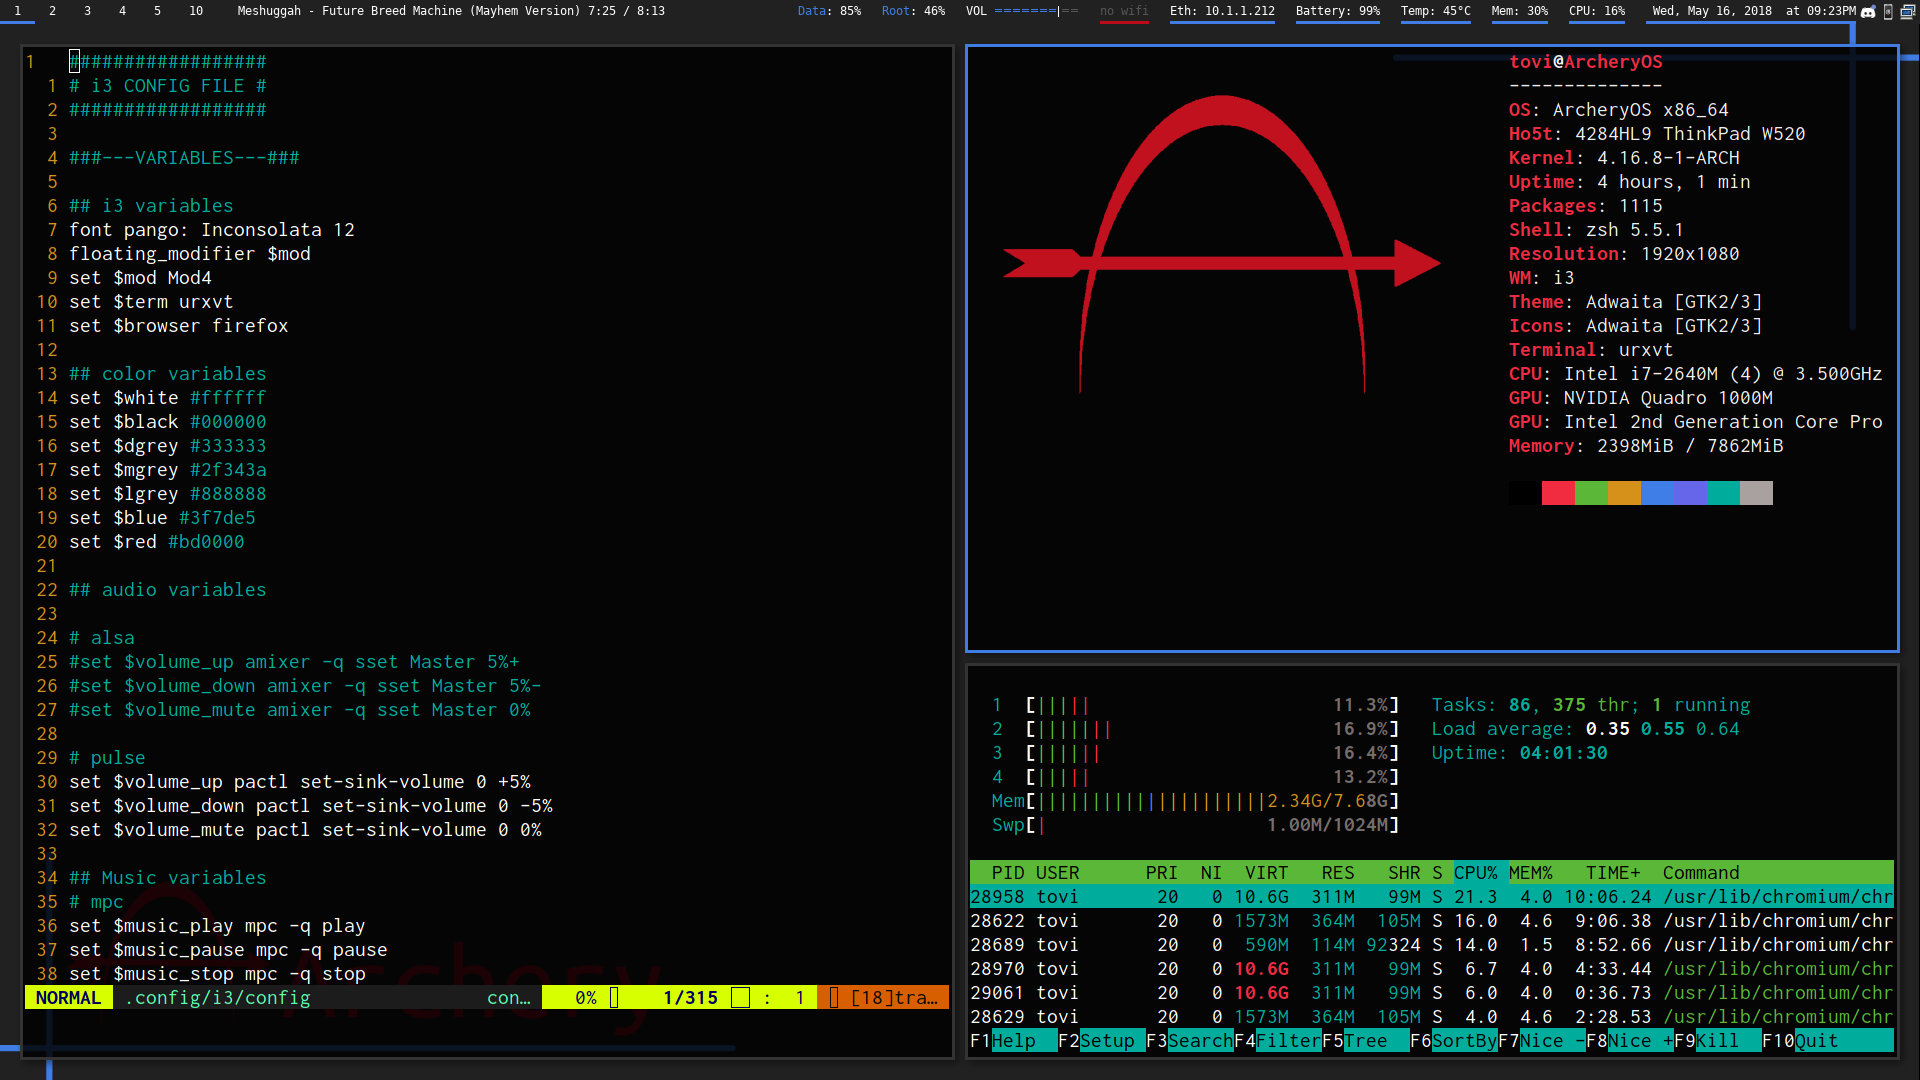
\includegraphics[width=\textwidth]{i3wm.png}
	\caption{i3 running vim, htop, and neofetch in 3 terminals}
\end{figure}
\end{center}
\section{i3}
\subsection{Introduction to i3}
``i3 is a tiling window manager, completely written from scratch. The target platforms are GNU/Linux and BSD operating systems, our code is Free and Open Source Software (FOSS) under the BSD license\. \i3 is primarily targeted at advanced users and developers.'' --- \textcite{i3wm}

\subsection{keybinds}
``Mod'' is a reference to the super key, what is known as the ``Windows key''.
Mod+F1 will show this document at any time
\subsubsection{i3 basics}
\begin{itemize}
	\item \textbf{Mod+Enter} --- Open a terminal window
	\item \textbf{Mod+Shift+Enter} --- Open a terminal window running tmux
	\item \textbf{Mod+q} --- Close active window
	\item \textbf{Mod+Shift+q} --- Close active window
	\item \textbf{Mod+Space} --- Toggles between a floating and non floating window
	\item \textbf{Mod+Shift+Space} --- Makes a tiled window into a floating window
	\item \textbf{Mod+Shift+r} --- Restart i3
	\item \textbf{Mod+d} --- rofi (a program launcher)
	\item \textbf{Mod+Shift+d} --- rofi in ``show window'' mode (allows user to navigate to running programs)
	\item \textbf{Mod+t} --- Toggle between spawning new windows horizontally or vertically to the active window
	\item \textbf{Mod+v} --- Spawn new windows vertically from active window
	\item \textbf{Mod+Shift+v} --- Spawn new windows horizontally from active window
	\item \textbf{Mod+f} --- Fullscreen
	\item \textbf{Mod+h} --- Move to window left of active window
	\item \textbf{Mod+Shift+h} --- Move active window left
	\item \textbf{Mod+j} --- Move to window below of active window
	\item \textbf{Mod+Shift+j} --- Move active window down
	\item \textbf{Mod+k} --- Move to window above of active window
	\item \textbf{Mod+Shift+k} --- Move active window up
	\item \textbf{Mod+l} --- Move to window right of active window
	\item \textbf{Mod+Shift+l} --- Move active window right
	\item \textbf{Mod+Shift+y} --- Expand active windows width by 10 px
	\item \textbf{Mod+Shift+u} --- Shrink active windows hight by 10px
	\item \textbf{Mod+Shift+i} --- Expand active windows hight by 10px
	\item \textbf{Mod+o} --- Opens a GUI program menu
	\item \textbf{Mod+Shift+o} --- Shrink active windows width by 10 px
	\item \textbf{Mod+e} --- Change to default layout
	\item \textbf{Mod+w} --- Change to tabbed layout
	\item \textbf{Mod+s} --- Change to stacked layout
	\item \textbf{Mod+Shift+s} --- Lock/logout/shutdown/reboot system
	\item \textbf{Mod+a} --- Focuses parent program
	\item \textbf{Mod+n} --- Expand outer gaps
	\item \textbf{Mod+Shift+n} --- Shrink outer gaps
	\item \textbf{Mod+g} --- Expand inner gaps
	\item \textbf{Mod+Shift+g} --- Shrink inner gaps
	\item \textbf{Mod+c} --- Sets gaps to default width
	\item \textbf{Mod+Shift+c} --- Turns off gaps
	\item \textbf{Mod+u} --- Next song
	\item \textbf{Mod+y} --- Previous song
\end{itemize}

\subsubsection{Programs}
\begin{itemize}
	\item \textbf{Mod+Shift+a} --- Audio (pavucontrol)
	\item \textbf{Mod+b} --- Browser (firefox)
	\item \textbf{Mod+i} --- System information (htop)
	\item \textbf{Mod+m} --- Music (ncmpcpp)
	\item \textbf{Mod+Shift+m} --- Mute audio
	\item \textbf{Mod+p} --- Play/pause music
	\item \textbf{Mod+Shift+p} --- Take screenshot (scrot)
	\item \textbf{Mod+r} --- File manager (ranger)
	\item \textbf{Mod+Shift+w} --- Newsboat
	\item \textbf{Mod+z} --- Toggle dropdown terminal
	\item \textbf{Mod+Shift+z} --- Reopen dropdown terminal (in case you accidentally close it)
\end{itemize}

\pagebreak

\section{Known bugs and issues}
\subsection{Screen size}
When first starting ArcheryOS in virtualbox, the screen size will be quite small. To fix this just logout and log back in again (\textbf{Mod+Shift+s} then \textbf{e}).
\subsection{Ranger image preview}
The default file manager in ArcheryOS, ranger, does not preview images when loaded in virtualbox. I have not found anyway to fix this, as of yet.

\subsection{Found more bugs?}
If you have found bugs or have any issuse with ArcheryOS, please submit an issue to \href{https://github.com/H0ll0wp0int/ArcheryOS-build-files}{the ArcheryOS github repo}.



\pagebreak
\section{Thanks}
Thank you to \textcite{Wallpape}, who created the wallpaper. See the bibliography for his github account.

\pagebreak
\printbibliography

\end{document}
